\PassOptionsToPackage{unicode=true}{hyperref} % options for packages loaded elsewhere
\PassOptionsToPackage{hyphens}{url}
\documentclass[11pt,dvipsnames,ignorenonframetext,aspectratio=169]{beamer}
\IfFileExists{pgfpages.sty}{\usepackage{pgfpages}}{}
\setbeamertemplate{caption}[numbered]
\setbeamertemplate{caption label separator}{: }
\setbeamercolor{caption name}{fg=normal text.fg}
\beamertemplatenavigationsymbolsempty
\usepackage{lmodern}
\usepackage{amssymb,amsmath}
\usepackage{ifxetex,ifluatex}
\usepackage{fixltx2e} % provides \textsubscript
\ifnum 0\ifxetex 1\fi\ifluatex 1\fi=0 % if pdftex
  \usepackage[T1]{fontenc}
  \usepackage[utf8]{inputenc}
\else % if luatex or xelatex
  \ifxetex
    \usepackage{mathspec}
  \else
    \usepackage{fontspec}
\fi
\defaultfontfeatures{Ligatures=TeX,Scale=MatchLowercase}







\fi

  \usetheme[]{monash}

  \usecolortheme{monashwhite}


% A default size of 24 is set in beamerthememonash.sty

% Title page
\setbeamertemplate{title page}
{\placefig{-0.01}{-0.01}{width=1.01\paperwidth,height=1.01\paperheight}{rhinocerousbeetle.jpg}
% \begin{textblock}{7.5}(1,2.8)\usebeamerfont{title} % original
\begin{textblock}{15}(1,2.2)\usebeamerfont{title}
{\color{white}\raggedright\par\inserttitle}
\end{textblock}
\begin{textblock}{10}(1,6)
\small
{\color{white}\raggedright{\insertauthor}\mbox{}\\[0.1cm]
\insertdate}
\end{textblock}}


  \useinnertheme{rounded}

  \useoutertheme{smoothtree}

% use upquote if available, for straight quotes in verbatim environments
\IfFileExists{upquote.sty}{\usepackage{upquote}}{}
% use microtype if available
\IfFileExists{microtype.sty}{%
  \usepackage{microtype}
  \UseMicrotypeSet[protrusion]{basicmath} % disable protrusion for tt fonts
}{}


\newif\ifbibliography


\hypersetup{
      pdftitle={Combining ability analysis},
            colorlinks=true,
    linkcolor=red,
    citecolor=Blue,
    urlcolor=lightgrayd,
    breaklinks=true}
%\urlstyle{same}  % Use monospace font for urls







% Prevent slide breaks in the middle of a paragraph:
\widowpenalties 1 10000
\raggedbottom

  \AtBeginPart{
    \let\insertpartnumber\relax
    \let\partname\relax
    \frame{\partpage}
  }
  \AtBeginSection{
    \ifbibliography
    \else
      \let\insertsectionnumber\relax
      \let\sectionname\relax
      \frame{\sectionpage}
    \fi
  }
  \AtBeginSubsection{
    \let\insertsubsectionnumber\relax
    \let\subsectionname\relax
    \frame{\subsectionpage}
  }



\setlength{\parindent}{0pt}
\setlength{\parskip}{6pt plus 2pt minus 1pt}
\setlength{\emergencystretch}{3em}  % prevent overfull lines
\providecommand{\tightlist}{%
  \setlength{\itemsep}{0pt}\setlength{\parskip}{0pt}}

  \setcounter{secnumdepth}{0}


%% Monash overrides
\AtBeginSection[]{
   \frame<beamer>{
   \frametitle{Outline}\vspace*{0.2cm}
   
   \tableofcontents[currentsection,hideallsubsections]
  }}

% Redefine shaded environment if it exists (to ensure text is black)
\ifcsname Shaded\endcsname
  \definecolor{shadecolor}{RGB}{225,225,225}
  \renewenvironment{Shaded}{\color{black}\begin{snugshade}\color{black}}{\end{snugshade}}
\fi
%%

  \usepackage{setspace}
  \usepackage{wasysym}
  % \usepackage{footnote} % don't use this this breaks all
  \usepackage{fontenc}
  \usepackage{fontawesome}
  \usepackage{booktabs,siunitx}
  \usepackage{longtable}
  \usepackage{array}
  \usepackage{multirow}
  \usepackage{wrapfig}
  \usepackage{float}
  \usepackage{colortbl}
  \usepackage{pdflscape}
  \usepackage{tabu}
  \usepackage{threeparttable}
  \usepackage{threeparttablex}
  \usepackage[normalem]{ulem}
  \usepackage{makecell}
  \usepackage{xcolor}
  \usepackage{tikz} % required for image opacity change
  \usepackage[absolute,overlay]{textpos} % for text formatting
  \usepackage{chemfig}
  \usepackage[skip=0.333\baselineskip]{caption}
  % \newcommand*{\AlignChar}[1]{\makebox[1ex][c]{\ensuremath{\scriptstyle#1}}}%

  % this font option is amenable for beamer
  \setbeamerfont{caption}{size=\tiny}
  \singlespacing
  \definecolor{lightgrayd}{gray}{0.95}
  \definecolor{skyblued}{rgb}{0.65, 0.6, 0.94}
  \definecolor{oranged}{RGB}{245, 145, 200}

  \newlength{\cslhangindent}
  \setlength{\cslhangindent}{1.5em}
  \newenvironment{cslreferences}%
    {\setlength{\parindent}{0pt}%
    \everypar{\setlength{\hangindent}{\cslhangindent}}\ignorespaces}%
    {\par}

  \title[]{Combining ability analysis}


  \author[
        Deependra Dhakal\\
College of Natural Resource Management\\
Agriculture and Forestry University\\
\textit{ddhakal.rookie@gmail.com}\\
\url{https://rookie.rbind.io}
    ]{Deependra Dhakal\\
College of Natural Resource Management\\
Agriculture and Forestry University\\
\textit{ddhakal.rookie@gmail.com}\\
\url{https://rookie.rbind.io}}


\date[
      
  ]{
    }

\begin{document}

% Hide progress bar and footline on titlepage
  \begin{frame}[plain]
  \titlepage
  \end{frame}


   \frame<beamer>{
   \frametitle{Outline}\vspace*{0.2cm}
   
   \tableofcontents[hideallsubsections]
  }

\hypertarget{mating-designs-brown2014plantbreeding}{%
\section{Mating designs (Brown, Caligari, and Campos
2014)}\label{mating-designs-brown2014plantbreeding}}

\begin{frame}{Mating designs (Brown, Caligari, and Campos 2014)}
\begin{itemize}
\tightlist
\item
  Concept based on early work of Louis de Vilmorin from the proposition
  he made that the only means to determine the value of an individual
  plant (or genotype) was to grow and evaluate its progeny -- A
  procedure known as \textbf{Progeny testing}.
\item
  Mating designs allow for partitioning of phenotypic effects -- as due
  to genotype, environment or interacting effects among genes and
  alleles.

  \begin{itemize}
  \tightlist
  \item
    identification of heterotic groups,
  \item
    estimation of general and specific combining abilities and
  \item
    testing of environmental interactions
  \end{itemize}
\item
  Selection methods can be stated as either being forward or backward.
  Forward selection is synonymous to \textbf{within-family selection}
  whereas the concept of backward selection embodies \textbf{selection
  among families}.
\item
  Forward selection works best for highly heritable traits -- for those
  traits regulated by few small genes, as opposed to those involving
  large number of genes with small cumulative effects.
\end{itemize}
\end{frame}

\begin{frame}{}
\protect\hypertarget{section}{}
\begin{itemize}
\tightlist
\item
  Selection gets more complicated as data on several different
  individuals belonging to some families is available.
\end{itemize}

\centering Expectation versus Reality

\begin{columns}[T,onlytextwidth]

\column{0.5\textwidth}


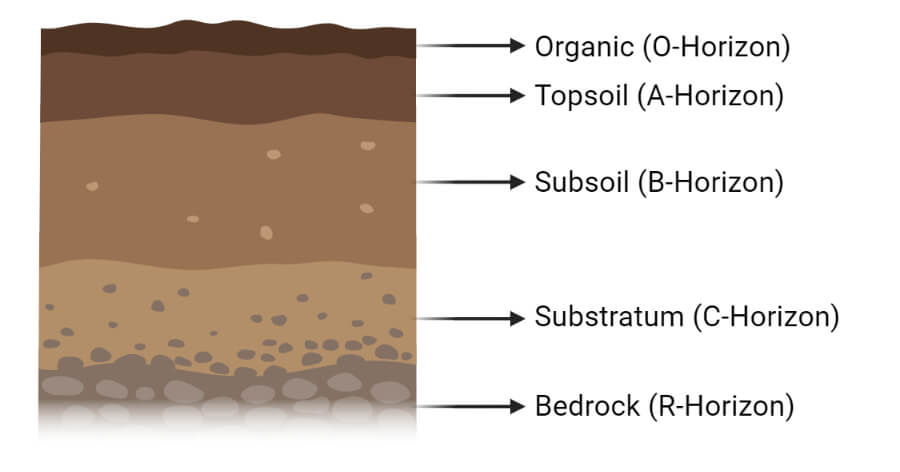
\includegraphics[width=0.8\linewidth]{../images/soil-profile-and-horizons} 

\column{0.5\textwidth}


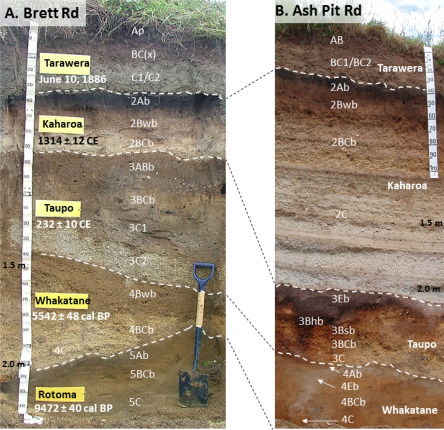
\includegraphics[width=0.8\linewidth]{../images/soil-profile-complex} 

\end{columns}
\end{frame}

\begin{frame}{}
\protect\hypertarget{section-1}{}
Broadly, three distinct modes of selection could be practiced:

\begin{enumerate}
\tightlist
\item
  Strict within family selection
\item
  Selection on within family deviation
\item
  Combined family and within family selection; family selection index
\end{enumerate}

\footnotesize

When the interest is to exploit the state of heterosis arising from
certain combination of parental individuals, the genetic factors
contributing well to superior phenotype should be underpinned. The whole
process of determining favorable combination among parental individuals
should be met with phenotypic data from many progeny, which is
retrospective in purpose -- thus the name backward (family) selection.

\begin{itemize}
\tightlist
\item
  Half-sib selection is used to select superier individuals for their
  GCA.
\item
  Full-sib selection is used to make distinct parental matings in order
  to induce hybrid vigor by capturing specific combinining abilities
\end{itemize}
\end{frame}

\begin{frame}{}
\protect\hypertarget{section-2}{}
The concept of combining abilities was first laid out by Sprague and
Tatum in 1942 (Sprague and Tatum 1942) in order to generate variance
estimates without too much of underlying genetic assumptions. The
combining ability test procedure involves making crossess of several
different combinations from a set of parents and ascribing the resultant
variances statistically to either the genetic additiveness of parental
charactersistics or the interacting parental genetic combinations. Thus,
the phenotype (\(y_i\)) of a cross progeny can be modeled as linear
combination of additive (\(A_i\)), dominance (\(D_i\)) and environmental
(\(e_i\)) effects, is:

\[y_i = \mu + A_i + D_i + e_i\]
\end{frame}

\begin{frame}{Combining ability}
\protect\hypertarget{combining-ability}{}
\begin{itemize}
\tightlist
\item
  This mean performance of a line, when expressed as a deviation from
  the mean of all crosses, gives what is called the general combining
  ability (\textbf{GCA}) of the lines.

  \begin{itemize}
  \tightlist
  \item
    Calculated as the average of all \(F_1\)s having this particular
    line as one parent
  \item
    Each cross has an expected value (the sum of GCAs of its two
    parental lines)
  \item
    Differences of GCA are due to the additive and additive x additive
    interactions in the base population
  \end{itemize}
\item
  The mean genotypic value of offspring from a particular cross may
  deviate from value expected considering the population mean and the
  sum of the parental GCA effects -- the specific combining ability
  (\textbf{SCA}) for that cross.

  \begin{itemize}
  \tightlist
  \item
    differences are attributable to nonadditive
    (inter-allelic/intra-loci interactions) genetic variance.
  \end{itemize}
\item
  SCA is expected to increase in variance more rapidly as inbreeding in
  the population reaches high levels.
\end{itemize}
\end{frame}

\begin{frame}{}
\protect\hypertarget{section-3}{}
\begin{itemize}
\tightlist
\item
  Mean genotypic value (\(G_{AB}\)) for the full-sib family produced by
  crossing parents A and B as the sum of the overall mean \(\mu\), the
  GCAs of the two parents and the SCA value:
\end{itemize}

\[G_{AB} = \mu + GCA_A + GCA_B + SCA_{AB}\]

\begin{itemize}
\tightlist
\item
  The types of interactions that can be obtained (SCA effects) depend
  upon the mating scheme used to produce the crosses, the most common
  being the diallel mating design, developed by B. Griffing (1956).
  Methods such as top cross and poly-cross are also not uncommon.
\end{itemize}
\end{frame}

\begin{frame}{}
\protect\hypertarget{section-4}{}
\begin{itemize}
\tightlist
\item
  A classical method to estimate dominance genetic variance (D) is to
  estimate the variance associated with SCA effects of many crosses.
\item
  Expected value of the observed SCA variance component is 1/4 of the
  dominance genetic variance in the reference population.
\item
  The GCA of each line is calculated as follows:
\end{itemize}

\[
\mathrm{G_x} = \left[\frac{T_x}{n-2}\right]-\left[\frac{\sum T}{n(n-2)}\right]
\]

\begin{itemize}
\tightlist
\item
  Where \(x\) represents a specific line.
\end{itemize}
\end{frame}

\begin{frame}{}
\protect\hypertarget{section-5}{}
Using fabricated dataset given in Table \ref{tab:fabricated-diallel}
following procedures outlines how GCA for Parent 2 (P2) (\(GCA_{P2}\))
can be calculated.

\begin{equation}
\begin{split}
\mathrm{G_b} & = \left[\frac{T_x}{n-2}\right]-\left[\frac{\sum T}{n(n-2)}\right] \\
 & = \left[\frac{39.7}{8}\right]-\left[\frac{324.7}{10\times 8}\right] \\
 & = 4.96-4.06 \\
 & = 0.9
\end{split}
\end{equation}
\end{frame}

\hypertarget{diallel-scheme}{%
\section{Diallel scheme}\label{diallel-scheme}}

\begin{frame}{}
\protect\hypertarget{section-6}{}
\begin{itemize}
\tightlist
\item
  Term \emph{diallel cross} was first used by Danish geneticist J.
  Schmidt in animal breeding work.
\item
  More sophisticated application of Vilmorin's progeny test.
\item
  Types of diallel mating design:
\end{itemize}
\end{frame}

\begin{frame}{}
\protect\hypertarget{section-7}{}
\begin{enumerate}
\tightlist
\item
  \textbf{Full/Complete diallels}: All the possible combinations of
  crosses among parents, including reciprocals and self-fertilization of
  the parents are made. For a sample of \(n\) parents, the full-diallel
  requires \(n \times n\) (\(n^2\)) progenies, a number that quickly
  becomes unmanageable as more parents are sampled (Table
  \ref{tab:full-diallel}).
\end{enumerate}

\begingroup\fontsize{8}{10}\selectfont

\begin{longtable}[t]{>{\raggedright\arraybackslash}p{3.0em}>{\raggedright\arraybackslash}p{3.0em}>{\raggedright\arraybackslash}p{3.0em}>{\raggedright\arraybackslash}p{3.0em}>{\raggedright\arraybackslash}p{3.0em}>{\raggedright\arraybackslash}p{3.0em}>{\raggedright\arraybackslash}p{3.0em}>{\raggedright\arraybackslash}p{3.0em}>{\raggedright\arraybackslash}p{3.0em}>{\raggedright\arraybackslash}p{3.0em}>{\raggedright\arraybackslash}p{3.5em}}
\caption{\label{tab:full-diallel}Full diallel mating scheme using 10 parents}\\
\toprule
Parents & P1 & P2 & P3 & P4 & P5 & P6 & P7 & P8 & P9 & P10\\
\midrule
\textbf{\cellcolor{gray!6}{P1}} & \cellcolor{gray!6}{P1 x P1} & \cellcolor{gray!6}{P1 x P2} & \cellcolor{gray!6}{P1 x P3} & \cellcolor{gray!6}{P1 x P4} & \cellcolor{gray!6}{P1 x P5} & \cellcolor{gray!6}{P1 x P6} & \cellcolor{gray!6}{P1 x P7} & \cellcolor{gray!6}{P1 x P8} & \cellcolor{gray!6}{P1 x P9} & \cellcolor{gray!6}{P1 x P10}\\
\textbf{P2} & P2 x P1 & P2 x P2 & P2 x P3 & P2 x P4 & P2 x P5 & P2 x P6 & P2 x P7 & P2 x P8 & P2 x P9 & P2 x P10\\
\textbf{\cellcolor{gray!6}{P3}} & \cellcolor{gray!6}{P3 x P1} & \cellcolor{gray!6}{P3 x P2} & \cellcolor{gray!6}{P3 x P3} & \cellcolor{gray!6}{P3 x P4} & \cellcolor{gray!6}{P3 x P5} & \cellcolor{gray!6}{P3 x P6} & \cellcolor{gray!6}{P3 x P7} & \cellcolor{gray!6}{P3 x P8} & \cellcolor{gray!6}{P3 x P9} & \cellcolor{gray!6}{P3 x P10}\\
\textbf{P4} & P4 x P1 & P4 x P2 & P4 x P3 & P4 x P4 & P4 x P5 & P4 x P6 & P4 x P7 & P4 x P8 & P4 x P9 & P4 x P10\\
\textbf{\cellcolor{gray!6}{P5}} & \cellcolor{gray!6}{P5 x P1} & \cellcolor{gray!6}{P5 x P2} & \cellcolor{gray!6}{P5 x P3} & \cellcolor{gray!6}{P5 x P4} & \cellcolor{gray!6}{P5 x P5} & \cellcolor{gray!6}{P5 x P6} & \cellcolor{gray!6}{P5 x P7} & \cellcolor{gray!6}{P5 x P8} & \cellcolor{gray!6}{P5 x P9} & \cellcolor{gray!6}{P5 x P10}\\
\addlinespace
\textbf{P6} & P6 x P1 & P6 x P2 & P6 x P3 & P6 x P4 & P6 x P5 & P6 x P6 & P6 x P7 & P6 x P8 & P6 x P9 & P6 x P10\\
\textbf{\cellcolor{gray!6}{P7}} & \cellcolor{gray!6}{P7 x P1} & \cellcolor{gray!6}{P7 x P2} & \cellcolor{gray!6}{P7 x P3} & \cellcolor{gray!6}{P7 x P4} & \cellcolor{gray!6}{P7 x P5} & \cellcolor{gray!6}{P7 x P6} & \cellcolor{gray!6}{P7 x P7} & \cellcolor{gray!6}{P7 x P8} & \cellcolor{gray!6}{P7 x P9} & \cellcolor{gray!6}{P7 x P10}\\
\textbf{P8} & P8 x P1 & P8 x P2 & P8 x P3 & P8 x P4 & P8 x P5 & P8 x P6 & P8 x P7 & P8 x P8 & P8 x P9 & P8 x P10\\
\textbf{\cellcolor{gray!6}{P9}} & \cellcolor{gray!6}{P9 x P1} & \cellcolor{gray!6}{P9 x P2} & \cellcolor{gray!6}{P9 x P3} & \cellcolor{gray!6}{P9 x P4} & \cellcolor{gray!6}{P9 x P5} & \cellcolor{gray!6}{P9 x P6} & \cellcolor{gray!6}{P9 x P7} & \cellcolor{gray!6}{P9 x P8} & \cellcolor{gray!6}{P9 x P9} & \cellcolor{gray!6}{P9 x P10}\\
\textbf{P10} & P10 x P1 & P10 x P2 & P10 x P3 & P10 x P4 & P10 x P5 & P10 x P6 & P10 x P7 & P10 x P8 & P10 x P9 & P10 x P10\\
\bottomrule
\end{longtable}
\endgroup{}
\end{frame}

\begin{frame}{}
\protect\hypertarget{section-8}{}
\begin{enumerate}
\setcounter{enumi}{1}
\tightlist
\item
  \textbf{Half diallels}: Each parent is mated with every other parent,
  excluding selfs and reciprocals. This requires making
  \(\frac{n(n-1)}{2}\) crosses for n parents (Table
  \ref{tab:half-diallel}).
\end{enumerate}

\begingroup\fontsize{8}{10}\selectfont

\begin{longtable}[t]{>{\raggedright\arraybackslash}p{3.0em}>{\raggedright\arraybackslash}p{3.0em}>{\raggedright\arraybackslash}p{3.0em}>{\raggedright\arraybackslash}p{3.0em}>{\raggedright\arraybackslash}p{3.0em}>{\raggedright\arraybackslash}p{3.0em}>{\raggedright\arraybackslash}p{3.0em}>{\raggedright\arraybackslash}p{3.0em}>{\raggedright\arraybackslash}p{3.0em}>{\raggedright\arraybackslash}p{3.0em}>{\raggedright\arraybackslash}p{3.0em}}
\caption{\label{tab:half-diallel}Half diallel mating scheme using 10 parents}\\
\toprule
Parents & P1 & P2 & P3 & P4 & P5 & P6 & P7 & P8 & P9 & P10\\
\midrule
\endfirsthead
\caption[]{Half diallel mating scheme using 10 parents \textit{(continued)}}\\
\toprule
Parents & P1 & P2 & P3 & P4 & P5 & P6 & P7 & P8 & P9 & P10\\
\midrule
\endhead

\endfoot
\bottomrule
\endlastfoot
\cellcolor{gray!6}{P1} & \cellcolor{gray!6}{} & \cellcolor{gray!6}{} & \cellcolor{gray!6}{} & \cellcolor{gray!6}{} & \cellcolor{gray!6}{} & \cellcolor{gray!6}{} & \cellcolor{gray!6}{} & \cellcolor{gray!6}{} & \cellcolor{gray!6}{} & \cellcolor{gray!6}{}\\
P2 & P2 x P1 &  &  &  &  &  &  &  &  & \\
\cellcolor{gray!6}{P3} & \cellcolor{gray!6}{P3 x P1} & \cellcolor{gray!6}{P3 x P2} & \cellcolor{gray!6}{} & \cellcolor{gray!6}{} & \cellcolor{gray!6}{} & \cellcolor{gray!6}{} & \cellcolor{gray!6}{} & \cellcolor{gray!6}{} & \cellcolor{gray!6}{} & \cellcolor{gray!6}{}\\
P4 & P4 x P1 & P4 x P2 & P4 x P3 &  &  &  &  &  &  & \\
\cellcolor{gray!6}{P5} & \cellcolor{gray!6}{P5 x P1} & \cellcolor{gray!6}{P5 x P2} & \cellcolor{gray!6}{P5 x P3} & \cellcolor{gray!6}{P5 x P4} & \cellcolor{gray!6}{} & \cellcolor{gray!6}{} & \cellcolor{gray!6}{} & \cellcolor{gray!6}{} & \cellcolor{gray!6}{} & \cellcolor{gray!6}{}\\
\addlinespace
P6 & P6 x P1 & P6 x P2 & P6 x P3 & P6 x P4 & P6 x P5 &  &  &  &  & \\
\cellcolor{gray!6}{P7} & \cellcolor{gray!6}{P7 x P1} & \cellcolor{gray!6}{P7 x P2} & \cellcolor{gray!6}{P7 x P3} & \cellcolor{gray!6}{P7 x P4} & \cellcolor{gray!6}{P7 x P5} & \cellcolor{gray!6}{P7 x P6} & \cellcolor{gray!6}{} & \cellcolor{gray!6}{} & \cellcolor{gray!6}{} & \cellcolor{gray!6}{}\\
P8 & P8 x P1 & P8 x P2 & P8 x P3 & P8 x P4 & P8 x P5 & P8 x P6 & P8 x P7 &  &  & \\
\cellcolor{gray!6}{P9} & \cellcolor{gray!6}{P9 x P1} & \cellcolor{gray!6}{P9 x P2} & \cellcolor{gray!6}{P9 x P3} & \cellcolor{gray!6}{P9 x P4} & \cellcolor{gray!6}{P9 x P5} & \cellcolor{gray!6}{P9 x P6} & \cellcolor{gray!6}{P9 x P7} & \cellcolor{gray!6}{P9 x P8} & \cellcolor{gray!6}{} & \cellcolor{gray!6}{}\\
P10 & P10 x P1 & P10 x P2 & P10 x P3 & P10 x P4 & P10 x P5 & P10 x P6 & P10 x P7 & P10 x P8 & P10 x P9 & \\*
\end{longtable}
\endgroup{}
\end{frame}

\begin{frame}{}
\protect\hypertarget{section-9}{}
\begin{enumerate}
\setcounter{enumi}{2}
\tightlist
\item
  \textbf{Partial diallel}: Not all the crosses are made. There are no
  reciprocals or selfs. The goal is to reduce the breeding workload for
  a given sample of parents by making less than \(\frac{n(n-1)}{2}\)
  crosses for n parents (Table \ref{tab:partial-diallel-10p-table} is
  for example diallel cross involving 10 parental lines and 7 set of
  cross involving each parent).
\end{enumerate}

With the partial scheme of diallel cross, same number of parents could
be tested in a framework with fewer crosses. The number of crosses in a
partial diallel scheme is given by,

\[
x = \frac{n \times s}{2}
\]

By analogy, we could have said that large number of lines could be
tested with lesser crossings under diallel scheme. Rearranging the above
relationship, \(\large n = \frac{2x}{s}\).
\end{frame}

\begin{frame}{}
\protect\hypertarget{section-10}{}
\begingroup\fontsize{8}{10}\selectfont

\begin{longtable}[t]{rllllllllll}
\caption{\label{tab:partial-diallel-10p-table}Partial diallel cross involving 10 parents combined in 7 set of crossess each.}\\
\toprule
p & 1 & 2 & 3 & 4 & 5 & 6 & 7 & 8 & 9 & 10\\
\midrule
\cellcolor{gray!6}{1} & \cellcolor{gray!6}{} & \cellcolor{gray!6}{} & \cellcolor{gray!6}{} & \cellcolor{gray!6}{4 x 1} & \cellcolor{gray!6}{5 x 1} & \cellcolor{gray!6}{6 x 1} & \cellcolor{gray!6}{7 x 1} & \cellcolor{gray!6}{8 x 1} & \cellcolor{gray!6}{} & \cellcolor{gray!6}{}\\
2 &  &  &  &  & 5 x 2 & 6 x 2 & 7 x 2 & 8 x 2 & 9 x 2 & \\
\cellcolor{gray!6}{3} & \cellcolor{gray!6}{} & \cellcolor{gray!6}{} & \cellcolor{gray!6}{} & \cellcolor{gray!6}{} & \cellcolor{gray!6}{} & \cellcolor{gray!6}{6 x 3} & \cellcolor{gray!6}{7 x 3} & \cellcolor{gray!6}{8 x 3} & \cellcolor{gray!6}{9 x 3} & \cellcolor{gray!6}{10 x 3}\\
4 &  &  &  &  &  &  & 7 x 4 & 8 x 4 & 9 x 4 & 10 x 4\\
\cellcolor{gray!6}{5} & \cellcolor{gray!6}{} & \cellcolor{gray!6}{} & \cellcolor{gray!6}{} & \cellcolor{gray!6}{} & \cellcolor{gray!6}{} & \cellcolor{gray!6}{} & \cellcolor{gray!6}{} & \cellcolor{gray!6}{8 x 5} & \cellcolor{gray!6}{9 x 5} & \cellcolor{gray!6}{10 x 5}\\
\addlinespace
6 &  &  &  &  &  &  &  &  & 9 x 6 & 10 x 6\\
\cellcolor{gray!6}{7} & \cellcolor{gray!6}{} & \cellcolor{gray!6}{} & \cellcolor{gray!6}{} & \cellcolor{gray!6}{} & \cellcolor{gray!6}{} & \cellcolor{gray!6}{} & \cellcolor{gray!6}{} & \cellcolor{gray!6}{} & \cellcolor{gray!6}{} & \cellcolor{gray!6}{10 x 7}\\
8 &  &  &  &  &  &  &  &  &  & \\
\cellcolor{gray!6}{9} & \cellcolor{gray!6}{} & \cellcolor{gray!6}{} & \cellcolor{gray!6}{} & \cellcolor{gray!6}{} & \cellcolor{gray!6}{} & \cellcolor{gray!6}{} & \cellcolor{gray!6}{} & \cellcolor{gray!6}{} & \cellcolor{gray!6}{} & \cellcolor{gray!6}{}\\
10 &  &  &  &  &  &  &  &  &  & \\
\bottomrule
\end{longtable}
\endgroup{}
\end{frame}

\hypertarget{analysis-of-diallel-cross}{%
\section{Analysis of diallel cross}\label{analysis-of-diallel-cross}}

\begin{frame}{}
\protect\hypertarget{section-11}{}
There are mainly two approaches for analysis and interpretation of data
derived from diallel cross. They are:

\begin{enumerate}
\tightlist
\item
  Analysis of general and specific combining ability. These methods are
  often referred to as Griffing's analyses, after B. Griffing who
  published his now famous paper \emph{Concept of general and specific
  combining ability in relation to diallel crossing systems}.
\item
  Analysis of array variances and covariances, often referred to as
  Hayman and Jinks' paper of 1953, \emph{The analysis of diallel
  crosses}
\end{enumerate}
\end{frame}

\begin{frame}{Griffing analysis}
\protect\hypertarget{griffing-analysis}{}
\footnotesize

Griffing's approach provides easy interpretation of results compared to
other analyses available. Parents used in diallel crosses can be
homozygous or heterozygous; for simplicity, diallel types are described
here in terms of homozygous (inbred) parents. Griffing's diallel
comprise of full diallel, half diallel (all possible combinations
without reciprocals but contains parental selfs), modified diallel (all
possible without parental selfs).

In simplest terms, the cross between two parents (i.e.~parent \(i\) and
parent \(j\)) in Griffing's analysis would be expressed as:

\[
X_{ij} = \mu + g_i + g_j + s_{ij}
\]

Where \(\mu\) is the overall mean of all entries in the diallel design,
\(g_i\) is the general combining ability of the \(i^{th}\) parent,
\(g_j\) is the general combining ability of the \(j^{th}\) parent, and
\(s_{ij}\) is the specific combining ability between the \(i_{th}\)
parent and the \(j_{th}\) parent.
\end{frame}

\begin{frame}{}
\protect\hypertarget{section-12}{}
General combining ability (GCA) measures the average performance of
parental lines in cross combination. GCA is therefore related to (but
not directly equal to) the proportion of variation that is genetically
additive in nature.

Specific combining ability (SCA) is the remaining part of the observed
phenotype that is not explained by the general combining ability of both
parents that constituted the progeny. By definition, SCA is the portion
of genetic variability which is not additive.
\end{frame}

\begin{frame}{}
\protect\hypertarget{section-13}{}
Griffing's analysis of a diallel is by analysis of variance, where the
total variance of all entries is partitioned into; and error variances.
In case where reciprocals are included, then reciprocals (or maternal
effects) are also partitioned. Error variances are estimated by
replication of families. To avoid excessive repetition, only Method 1
(complete diallel) and Method 2 (half diallel), both including parents,
will be considered further.
\end{frame}

\begin{frame}{}
\protect\hypertarget{section-14}{}
\footnotesize

Degrees of freedom (df), sum of squares (SS) and mean squares (MSq) from
the analysis of variance for Method 1 for the assumption of model 1
(fixed effects) are shown in Table \ref{tab:complete-diallel-fixed}

\begin{table}

\caption{\label{tab:complete-diallel-fixed}Degrees of freedom, sum of squares and mean squares from the analysis of variance of a full diallel including parent selfs (Method 1) assuming fixed effects. Also shown are the expectations for the mean squares}
\centering
\fontsize{8}{10}\selectfont
\begin{tabular}[t]{lllll}
\toprule
Source & df & SS & Msq & EMS\\
\midrule
GCA & p-1 & $S_g$ & $M_g$ & $\sigma^2 + 2p(1/(1-p))\sum g^2_i$\\
SCA & $\frac{p(p-1)}{2}$ & $S_s$ & $M_s$ & $\sigma^2 + \frac{2}{p(p-1)}\sum_{ij}s_{ij}^2$\\
Reciprocal & $\frac{p(p-1)}{2}$ & $S_r$ & $M_r$ & $\sigma^2 + 2\frac{2}{p(p-1)}\sum_{i<j}r_{ij}^2$\\
Error & $(r-1)p^2$ & $S_e$ & $M_e$ & $\sigma^2$\\
\bottomrule
\end{tabular}
\end{table}

that is, sum over rows; \(X_j\) is
\(\sum_ix_{ij} = x_{1j} + x_{2j} + x_{3j} + ...,\) that is, sum over
columns; and \(X_{...}\) is \(\sum_{ij}x_{ij}\), the sum of all
observations. Where r is the number of replicates; p is the numeber of
parents; \(S_g\) is
\(\frac{1}{p+2}(\sum_i(X_i + x_ii)^2-\frac{4}{pX_{...}^2})\); \(S_s\) is
\(\sum_{i<j}x_{ij}^2-\frac{1}{p+2}\sum_i(X_i + x_{ii})^2 + \frac{2}{(p+1)(P+2)X_{...}^2}\)
and \(X_{i...}\) is \(\sum_j x_{ij} = x_{i1} + x_{i2} + x_{i3} + ...,\)
that is, the sum over rows; \(X_{...}\) is \(\sum_{ij}x_{ij}\), the sum
of all observations.
\end{frame}

\begin{frame}{}
\protect\hypertarget{section-15}{}
\footnotesize

When SCA is relatively small in comparision with GCA, it should be
possible to predict the performance of particular cross combinations
based only on the values obtained for GCA of parents.

A realtively large SCA/GCA ratio implies the presence of dominance
and/or epistatic gene effects. It should be noted that if dominance x
additive effects are present, the GCA component will also contain some
of these effects in addition to pure additive effects.

For inbred lines, the closer that the following equations are equal to
one (i.e.~as SCA becomes small or very small compared with GCA), then
greater predictability based on GCA will be possible. The ratio
equations for each model are:

\[
\begin{aligned}
Model~1 &: \frac{2g_i^2}{[2g_i^2 + s_{ij}^2]} \\
Model~2 &: \frac{2\sigma_g^2}{[2\sigma_g^2 + \sigma_s^2]}
\end{aligned}
\]

Where \(g_i^2\), \(\sigma_g^2\) are the general combining ability mean
square and variance, respectively and \(s_{ij}\) and \(\sigma_s^2\) are
specific combining ability mean square and variance, respectively.
\end{frame}

\hypertarget{example-fabricated-diallel-cross-data}{%
\section{Example (fabricated) diallel cross
data}\label{example-fabricated-diallel-cross-data}}

\begin{frame}{}
\protect\hypertarget{section-16}{}
\begingroup\fontsize{8}{10}\selectfont

\begin{longtable}[t]{>{\raggedright\arraybackslash}p{3em}>{\raggedleft\arraybackslash}p{3em}>{\raggedleft\arraybackslash}p{3em}>{\raggedleft\arraybackslash}p{3em}>{\raggedleft\arraybackslash}p{3em}>{\raggedleft\arraybackslash}p{3em}>{\raggedleft\arraybackslash}p{3em}>{\raggedleft\arraybackslash}p{3em}>{\raggedleft\arraybackslash}p{3em}>{\raggedleft\arraybackslash}p{3em}>{\raggedleft\arraybackslash}p{3em}}
\caption{\label{tab:fabricated-diallel}Fabricated data from a diallel cross scheme using 10 parents}\\
\toprule
Parents & P1 & P2 & P3 & P4 & P5 & P6 & P7 & P8 & P9 & P10\\
\midrule
\textbf{\cellcolor{gray!6}{P1}} & \cellcolor{gray!6}{} & \cellcolor{gray!6}{} & \cellcolor{gray!6}{} & \cellcolor{gray!6}{} & \cellcolor{gray!6}{} & \cellcolor{gray!6}{} & \cellcolor{gray!6}{} & \cellcolor{gray!6}{} & \cellcolor{gray!6}{} & \cellcolor{gray!6}{}\\
\textbf{P2} & 2.8 &  &  &  &  &  &  &  &  & \\
\textbf{\cellcolor{gray!6}{P3}} & \cellcolor{gray!6}{2.1} & \cellcolor{gray!6}{2.0} & \cellcolor{gray!6}{} & \cellcolor{gray!6}{} & \cellcolor{gray!6}{} & \cellcolor{gray!6}{} & \cellcolor{gray!6}{} & \cellcolor{gray!6}{} & \cellcolor{gray!6}{} & \cellcolor{gray!6}{}\\
\textbf{P4} & 2.3 & 3.8 & 1.12 &  &  &  &  &  &  & \\
\textbf{\cellcolor{gray!6}{P5}} & \cellcolor{gray!6}{3.4} & \cellcolor{gray!6}{4.4} & \cellcolor{gray!6}{1.80} & \cellcolor{gray!6}{5.0} & \cellcolor{gray!6}{} & \cellcolor{gray!6}{} & \cellcolor{gray!6}{} & \cellcolor{gray!6}{} & \cellcolor{gray!6}{} & \cellcolor{gray!6}{}\\
\addlinespace
\textbf{P6} & 3.6 & 3.2 & 0.55 & 6.3 & 3.8 &  &  &  &  & \\
\textbf{\cellcolor{gray!6}{P7}} & \cellcolor{gray!6}{2.3} & \cellcolor{gray!6}{2.5} & \cellcolor{gray!6}{2.00} & \cellcolor{gray!6}{4.6} & \cellcolor{gray!6}{3.4} & \cellcolor{gray!6}{3.1} & \cellcolor{gray!6}{} & \cellcolor{gray!6}{} & \cellcolor{gray!6}{} & \cellcolor{gray!6}{}\\
\textbf{P8} & 2.7 & 2.9 & 0.89 & 2.4 & 2.1 & 4.4 & 4.9 &  &  & \\
\textbf{\cellcolor{gray!6}{P9}} & \cellcolor{gray!6}{3.1} & \cellcolor{gray!6}{3.5} & \cellcolor{gray!6}{2.11} & \cellcolor{gray!6}{0.9} & \cellcolor{gray!6}{3.6} & \cellcolor{gray!6}{3.8} & \cellcolor{gray!6}{5.3} & \cellcolor{gray!6}{3.9} & \cellcolor{gray!6}{} & \cellcolor{gray!6}{}\\
\textbf{P10} & 4.9 & 5.8 & 2.16 & 3.4 & 7.1 & 6.8 & 3.8 & 4.0 & 2.9 & \\
\bottomrule
\end{longtable}
\endgroup{}

\footnotesize

Taking the above table of diallel cross data, total of each individual
parental line could be computed by summing over all the crossess
involving the common parent. Similarly, the grand totals could be
obtained by adding together all the individual parents' total. The
individual parents' sum and grand total is shown in the Table
\ref{tab:sum-over-ind} below.
\end{frame}

\begin{frame}{}
\protect\hypertarget{section-17}{}
\begin{table}

\caption{\label{tab:sum-over-ind}Totals of individual lines and grand total of diallel cross
 scheme using 10 parents}
\centering
\fontsize{8}{10}\selectfont
\begin{tabular}[t]{>{}lr}
\toprule
Parents & Line total\\
\midrule
\textbf{\cellcolor{gray!6}{P1}} & \cellcolor{gray!6}{27}\\
\textbf{P2} & 31\\
\textbf{\cellcolor{gray!6}{P3}} & \cellcolor{gray!6}{15}\\
\textbf{P4} & 30\\
\textbf{\cellcolor{gray!6}{P5}} & \cellcolor{gray!6}{35}\\
\addlinespace
\textbf{P6} & 36\\
\textbf{\cellcolor{gray!6}{P7}} & \cellcolor{gray!6}{32}\\
\textbf{P8} & 28\\
\textbf{\cellcolor{gray!6}{P9}} & \cellcolor{gray!6}{29}\\
\textbf{P10} & 41\\
\addlinespace
\textbf{\cellcolor{gray!6}{Total}} & \cellcolor{gray!6}{303}\\
\bottomrule
\end{tabular}
\end{table}
\end{frame}

\hypertarget{bibliography}{%
\section{Bibliography}\label{bibliography}}

\begin{frame}{References}
\protect\hypertarget{references}{}
\hypertarget{refs}{}
\begin{cslreferences}
\leavevmode\hypertarget{ref-brown2014plantbreeding}{}%
Brown, Jack, Peter Caligari, and Hugo Campos. 2014. \emph{Plant
Breeding}. Wiley Blackwell.

\leavevmode\hypertarget{ref-sprague1942general}{}%
Sprague, George F, and Loyd A Tatum. 1942. ``General Vs. Specific
Combining Ability in Single Crosses of Corn 1.'' \emph{Agronomy Journal}
34 (10): 923--32.
\end{cslreferences}
\end{frame}




\end{document}
